\section{Methodology: The Magic Gem Framework}
\label{sec:methodology}

We now develop the Magic Gem framework, beginning with the construction of three-dimensional point clouds 
from magic squares and culminating in our main theoretical result connecting magic squares to zero-covariance configurations.

\subsection{From Magic Square to Point Cloud}

Let $S = (s_{ij})$ be an $n \times n$ magic square with entries $s_{ij} \in \{1, 2, \ldots, n^2\}$.
We construct a point cloud $P \subset \R^3$ by assigning three-dimensional coordinates to each cell of the grid.

\begin{definition}[Magic Gem Coordinates]
\label{def:gem_coords}
For each cell $(i, j)$ with $i, j \in \{0, 1, \ldots, n-1\}$, define the point
\begin{equation}
\mathbf{p}_{ij} = \left( x_{ij}, y_{ij}, z_{ij} \right),
\end{equation}
where the coordinates are given by
\begin{align}
x_{ij} &= j - \frac{n-1}{2}, \label{eq:x_coord} \\
y_{ij} &= \frac{n-1}{2} - i, \label{eq:y_coord} \\
z_{ij} &= s_{ij} - \frac{n^2 + 1}{2}. \label{eq:z_coord}
\end{align}
\end{definition}

The horizontal coordinates $x$ and $y$ place the grid centered at the origin,
with the $x$-axis aligned with columns and the $y$-axis aligned with rows (inverted so that the top row has positive $y$).
For a $3 \times 3$ grid, the nine positions have $x$- and $y$-coordinates in $\{-1, 0, 1\}$;
for a $5 \times 5$ grid, they lie in $\{-2, -1, 0, 1, 2\}$.

The vertical coordinate $z$ encodes the cell's value, shifted so that the mean value $(n^2 + 1)/2$ maps to zero.
This centering ensures that the point cloud has zero mean in all three coordinates,
a property that will prove essential for the covariance analysis.

\begin{example}[Lo Shu Square]
For the Lo Shu square
\[
S = \begin{pmatrix}
2 & 7 & 6 \\
9 & 5 & 1 \\
4 & 3 & 8
\end{pmatrix},
\]
with $n = 3$ and center value $5$, the nine points are
\begin{align*}
\mathbf{p}_{00} &= (-1, 1, -3), & \mathbf{p}_{01} &= (0, 1, 2), & \mathbf{p}_{02} &= (1, 1, 1), \\
\mathbf{p}_{10} &= (-1, 0, 4), & \mathbf{p}_{11} &= (0, 0, 0), & \mathbf{p}_{12} &= (1, 0, -4), \\
\mathbf{p}_{20} &= (-1, -1, -1), & \mathbf{p}_{21} &= (0, -1, -2), & \mathbf{p}_{22} &= (1, -1, 3).
\end{align*}
Note that the center cell, containing the value 5, maps to the origin.
\end{example}

\Cref{fig:construction} illustrates the four-step construction process, 
progressing from the magic square through the centered grid to the final three-dimensional representation,
along with all eight $D_4$ symmetry variants of the Lo Shu square.

\begin{figure}[H]
    \centering
    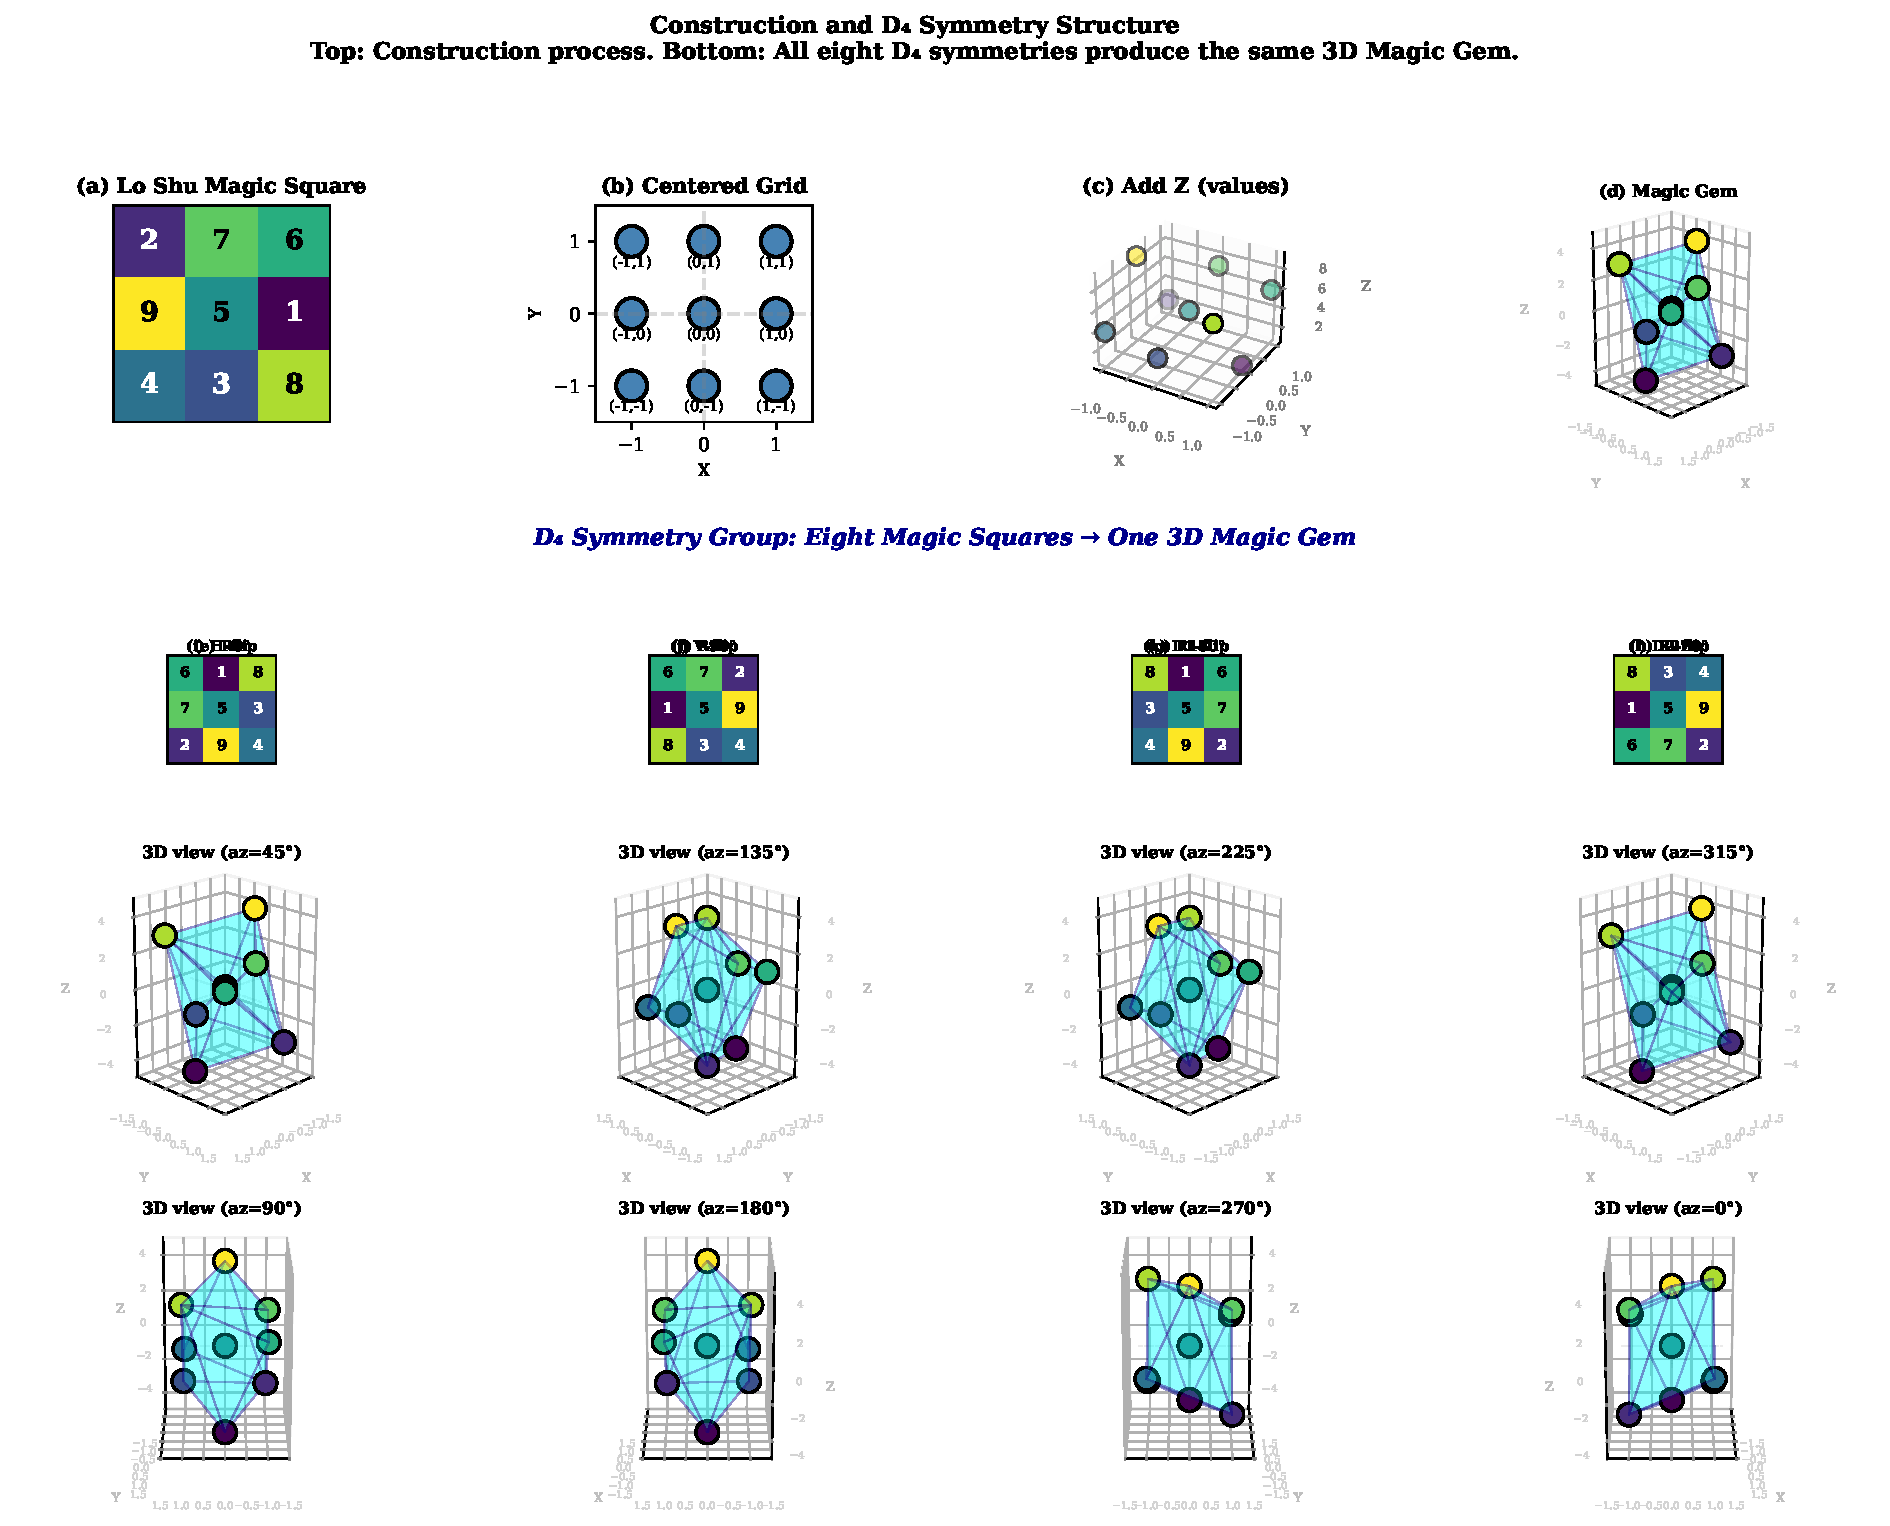
\includegraphics[width=\textwidth]{figures/fig02_combined_construction_symmetries.pdf}
    \caption{\textbf{Construction process and $D_4$ symmetry structure.}
    \emph{Top row (a--d):} Construction of a Magic Gem from the Lo Shu square.
    (a) The Lo Shu magic square---the unique (up to symmetry) $3 \times 3$ magic square, 
    with each row, column, and diagonal summing to $M(3) = 15$.
    (b) Placement on a centered coordinate grid with origin at center.
    (c) Assignment of $z$-values from cell entries.
    (d) Centered Magic Gem point cloud with convex hull.
    \emph{Bottom section (e--l):} The eight $D_4$ symmetries of the $3 \times 3$ magic square.
    Each panel shows a compact 2D magic square (top) paired with its corresponding 3D Magic Gem (bottom, large and prominent).
    The gems are shown from different viewing angles to emphasize their three-dimensional structure.
    Despite their distinct numerical arrangements, all eight $D_4$ variants yield the same 3D Magic Gem polyhedron,
    demonstrating the geometric invariance of the Magic Gem representation under the symmetry group.}
    \label{fig:construction}
\end{figure}

\subsection{The Magic Gem Polyhedron}

With the point cloud defined, we construct the Magic Gem as its convex hull \cite{barvinok2002course}.

\begin{definition}[Magic Gem]
The \emph{Magic Gem} associated with a magic square $S$ is the convex hull of the corresponding point cloud:
\[
\mathcal{G}(S) = \text{conv}\left( \{ \mathbf{p}_{ij} : 0 \leq i, j < n \} \right).
\]
\end{definition}

A fundamental property of this construction is its invariance under the symmetry operations of the magic square.

\begin{proposition}[Symmetry Invariance]
\label{prop:symmetry_invariance}
If $S'$ is obtained from $S$ by a symmetry operation $g \in D_4$, then $\mathcal{G}(S) = \mathcal{G}(S')$.
\end{proposition}

\begin{proof}
Each element $g \in D_4$ acts on the grid as an orthogonal transformation of the $(x, y)$ plane,
which extends naturally to an isometry of $\R^3$ that fixes the $z$-axis direction.
Under this action, the $z$-coordinates are permuted according to the relabeling of cells,
but the set of $z$-values remains unchanged.
Since convex hulls are invariant under isometries and depend only on the set of points (not their labeling),
we have $\mathcal{G}(S) = \mathcal{G}(S')$.
\end{proof}

This invariance means that all eight $D_4$ variants of a magic square produce the same Magic Gem.
For $n = 3$, this implies that the single essentially different magic square yields a unique Magic Gem,
while for larger orders, each equivalence class corresponds to a distinct geometric object.

The construction figure (\Cref{fig:construction}, bottom rows) displays all eight symmetry variants of the $3 \times 3$ magic square,
illustrating how these numerically distinct arrangements share a common geometric representation.

\subsection{The Vector Representation}
\label{sec:vector_rep}

The centering of our coordinate system invites an interpretation of each point as a vector from the origin.
Since the origin coincides with the centroid of the point cloud (as we shall verify),
this vector representation captures the deviation of each cell from the ``balanced'' center.

\begin{definition}[Magic Gem Vectors]
The \emph{vector representation} of a Magic Gem is the collection
\[
\mathcal{V}(S) = \left\{ \mathbf{v}_{ij} = \mathbf{p}_{ij} : 0 \leq i, j < n \right\},
\]
where each point is interpreted as a vector emanating from the origin.
\end{definition}

This interpretation connects the Magic Gem to the classical physics of rigid bodies:
if unit masses are placed at each vertex, the resulting configuration has its center of mass at the origin,
and the vectors $\mathbf{v}_{ij}$ describe the displacement of each mass from this center.

\subsubsection{Vectors and Covariance}

The vector representation provides a geometric interpretation of the zero-covariance condition.
Consider the weighted sum of vectors where each vector is weighted by its $x$-coordinate:
\[
\sum_{i,j} x_{ij} \mathbf{v}_{ij} = \sum_{i,j} x_{ij} (x_{ij}, y_{ij}, z_{ij}).
\]
The $z$-component of this weighted sum is precisely $n^2 \cdot \Cov(X, Z)$.
Thus, zero covariance is equivalent to the statement that vectors, 
when weighted by their horizontal positions, have no net vertical tendency.

More explicitly, define the \emph{position-weighted vector sums}:
\begin{align}
\mathbf{W}_x &= \sum_{i,j} x_{ij} \mathbf{v}_{ij}, \label{eq:weighted_x} \\
\mathbf{W}_y &= \sum_{i,j} y_{ij} \mathbf{v}_{ij}. \label{eq:weighted_y}
\end{align}
Then $\Cov(X, Z) = 0$ if and only if $(\mathbf{W}_x)_z = 0$, 
and $\Cov(Y, Z) = 0$ if and only if $(\mathbf{W}_y)_z = 0$.

This formulation reveals that magic squares achieve a form of \emph{directional balance}:
the $z$-values are distributed so that neither horizontal direction 
exhibits any systematic correlation with value magnitude.
The vectors in Figure panels showing the vector representation 
visually manifest this balance---vectors pointing in each horizontal direction 
have $z$-components that ``cancel out'' when weighted by position.

\subsection{The Covariance Structure of Magic Squares}
\label{sec:zero_cov_theorem}

We now establish our main theoretical results, revealing a deep connection 
between the algebraic definition of magic squares and the statistical structure of Magic Gems.

\subsubsection{Forward Direction: Magic Implies Zero Covariance}

The following result holds for all $n \geq 3$ and admits a clean algebraic proof.

\begin{proposition}[Magic Implies Zero Covariance]
\label{prop:magic_implies_zero_cov}
Let $S$ be an $n \times n$ magic square, and let $P = \{\mathbf{p}_{ij}\}$ be the corresponding point cloud. 
Then $\Cov(X, Z) = \Cov(Y, Z) = 0$.
\end{proposition}

\begin{proof}
We first verify that the means of all three coordinates vanish.
For the $x$-coordinate,
\[
\bar{X} = \frac{1}{n^2} \sum_{i,j} x_{ij} = \frac{1}{n^2} \sum_{i,j} \left( j - \frac{n-1}{2} \right) 
= \frac{n}{n^2} \sum_{j=0}^{n-1} \left( j - \frac{n-1}{2} \right) = 0,
\]
since $\sum_{j=0}^{n-1} j = n(n-1)/2$. An analogous argument shows $\bar{Y} = 0$, and 
\[
\bar{Z} = \frac{1}{n^2} \sum_{i,j} \left( s_{ij} - \frac{n^2+1}{2} \right) = 0
\]
since the entries sum to $n^2(n^2+1)/2$.

With zero means, $\Cov(X, Z) = \frac{1}{n^2} \sum_{i,j} x_{ij} z_{ij}$.
Define $C_j = \sum_{i=0}^{n-1} s_{ij}$ as the sum of column $j$. Then:
\[
\Cov(X, Z) = \frac{1}{n^2} \sum_{j=0}^{n-1} \left( j - \frac{n-1}{2} \right) C_j.
\]
For a magic square, all column sums equal $M(n)$, so
\[
\Cov(X, Z) = \frac{M(n)}{n^2} \sum_{j=0}^{n-1} \left( j - \frac{n-1}{2} \right) = 0.
\]
The argument for $\Cov(Y, Z) = 0$ via row sums is analogous.
\end{proof}

\begin{corollary}
For any magic square, the covariance matrix of the Magic Gem coordinates has the block-diagonal form
\[
\Sigma = \begin{pmatrix}
\Var(X) & \Cov(X,Y) & 0 \\
\Cov(X,Y) & \Var(Y) & 0 \\
0 & 0 & \Var(Z)
\end{pmatrix}.
\]
In particular, the $z$-coordinate is uncorrelated with both horizontal coordinates.
\end{corollary}

\subsubsection{On the Insufficiency of Aggregate Covariances}
\label{sec:insufficiency}

It is natural to ask whether the conditions $\Cov(X, Z) = \Cov(Y, Z) = 0$ alone 
suffice to characterize magic squares, or at least semi-magic squares 
(those with equal row and column sums but possibly failing the diagonal conditions).
Perhaps surprisingly, the answer is \emph{no}---and understanding why reveals 
a crucial distinction that motivates our energy functional approach.

\begin{remark}[Why $\Cov(X,Z)=0$ Is Not Enough]
\label{rem:first_moment}
The condition $\Cov(X, Z) = 0$ is equivalent to a single \emph{first-moment} constraint on column sums.
Let $C_j = \sum_{i=0}^{n-1} s_{ij}$ denote the sum of column $j$, and let $\delta_j = C_j - M(n)$ 
be the deviation from the magic constant. Then $\Cov(X, Z) = 0$ is equivalent to
\[
\sum_{j=0}^{n-1} \left( j - \frac{n-1}{2} \right) \delta_j = 0.
\]
Combined with the constraint $\sum_j \delta_j = 0$ (which follows from the total sum being fixed),
this leaves an $(n-2)$-dimensional space of possible deviation patterns.
For $n = 3$, the nonzero deviations must have the form $(\delta_0, \delta_1, \delta_2) = t(1, -2, 1)$;
for $n \geq 4$, the space of ``balanced but unequal'' column patterns grows rapidly.
\end{remark}

\begin{remark}[Counterexamples Exist for $n = 3$]
\label{rem:counterexample}
Exhaustive enumeration for $n = 3$ reveals that \emph{760 arrangements} of $\{1, \ldots, 9\}$ 
satisfy both $\Cov(X, Z) = 0$ and $\Cov(Y, Z) = 0$, yet only 8 of these are magic squares.
For instance, the arrangement
\[
S = \begin{pmatrix}
1 & 3 & 9 \\
8 & 6 & 5 \\
7 & 4 & 2
\end{pmatrix}
\]
has row sums $(13, 19, 13)$ and column sums $(16, 13, 16)$---far from equal---yet 
achieves $\Cov(X, Z) = \Cov(Y, Z) = 0$ exactly.
\end{remark}

\begin{remark}[The Four-Term Energy Is Insufficient for $n \geq 4$]
\label{rem:four_term_insufficient}
Even more strikingly, adding the diagonal covariance conditions does not resolve the issue for $n \geq 4$.
The four covariances $\Cov(X, Z)$, $\Cov(Y, Z)$, $\Cov(D_{\mathrm{main}}, Z)$, $\Cov(D_{\mathrm{anti}}, Z)$
impose only four linear constraints on the $(n^2 - 1)$-dimensional space of mean-zero value functions.
For $n = 4$, this leaves an $(n^2 - 5) = 11$-dimensional nullspace.

Consequently, there exist $4 \times 4$ permutations with all four covariances equal to zero 
that are \emph{not} magic squares. For example:
\[
S = \begin{pmatrix}
9 & 4 & 12 & 3 \\
16 & 1 & 14 & 7 \\
10 & 15 & 11 & 8 \\
2 & 5 & 6 & 13
\end{pmatrix}
\]
has both diagonal sums equal to $34$, but row sums $(28, 38, 44, 26)$ and column sums $(37, 25, 43, 31)$.
All four covariances vanish, yet the arrangement is not magic.
\end{remark}

This analysis reveals that aggregate position coordinates $X$ and $Y$ are too coarse:
they capture only the \emph{first moment} of the row and column sum distributions.
A true characterization requires testing against \emph{individual} row and column indicators,
which we develop in \Cref{sec:energy_landscape}.

\subsection{Diagonal Conditions as Covariances}
\label{sec:diagonal_cov}

The row and column constraints can be elegantly expressed via covariance with position coordinates.
We extend this framework to diagonal constraints by introducing indicator random variables.

\begin{definition}[Diagonal Indicators]
Define indicator variables for the main and anti-diagonals:
\begin{align}
D_{\mathrm{main}}(i,j) &= \begin{cases} 1 & \text{if } i = j, \\ 0 & \text{otherwise}, \end{cases} \\
D_{\mathrm{anti}}(i,j) &= \begin{cases} 1 & \text{if } i + j = n - 1, \\ 0 & \text{otherwise}. \end{cases}
\end{align}
\end{definition}

These indicators allow us to express diagonal constraints in covariance form.

\begin{proposition}[Diagonal Covariance Characterization]
\label{prop:diagonal_cov}
For an arrangement $S$ with centered $z$-values:
\begin{enumerate}
\item $\Cov(D_{\mathrm{main}}, Z) = 0$ if and only if the main diagonal sum equals $M(n)$.
\item $\Cov(D_{\mathrm{anti}}, Z) = 0$ if and only if the anti-diagonal sum equals $M(n)$.
\end{enumerate}
\end{proposition}

\begin{proof}
The mean of $D_{\mathrm{main}}$ over all cells is $\bar{D}_{\mathrm{main}} = n/n^2 = 1/n$.
With $\bar{Z} = 0$, we have:
\[
\Cov(D_{\mathrm{main}}, Z) = \frac{1}{n^2} \sum_{i,j} D_{\mathrm{main}}(i,j) \cdot z_{ij} - \bar{D}_{\mathrm{main}} \cdot \bar{Z}
= \frac{1}{n^2} \sum_{i=0}^{n-1} z_{ii}.
\]
Since $z_{ii} = s_{ii} - (n^2+1)/2$, the sum $\sum_i z_{ii} = \sum_i s_{ii} - n(n^2+1)/2$.
This vanishes if and only if $\sum_i s_{ii} = M(n)$. The anti-diagonal case is analogous.
\end{proof}

This reformulation expresses the diagonal constraints in the same statistical language as the row/column constraints.
Together with the aggregate position covariances $\Cov(X,Z)$ and $\Cov(Y,Z)$, these diagonal covariances define the
four-term ``low-mode'' energy $E_{\mathrm{low}}$ (\Cref{def:lowmode_energy}).
For $n=3$, $E_{\mathrm{low}}(S)=0$ is already sufficient to characterize magic squares
(verified by exhaustive enumeration; \Cref{prop:lowmode_char}),
but for $n\ge 4$ it is only a necessary relaxation (see \Cref{rem:four_term_insufficient}).
A complete characterization requires testing against individual row and column indicators, developed in \Cref{sec:energy_landscape}.

\subsection{Perturbation Analysis}
\label{sec:perturbation}

The zero-covariance characterization suggests that magic squares occupy special positions 
in the space of all arrangements.
We formalize this intuition through perturbation analysis.

\begin{proposition}[Local Optimality]
\label{prop:local_opt}
Let $S$ be a magic square with corresponding point cloud $P$, 
and let $\tilde{P}$ be obtained by perturbing the $z$-coordinates by amounts $\epsilon_{ij}$.
Define the off-diagonal covariance magnitude
\[
\Phi(\tilde{P}) = \Cov(X, \tilde{Z})^2 + \Cov(Y, \tilde{Z})^2.
\]
Then $\Phi(P) = 0$, and for generic perturbations $\epsilon$, we have $\Phi(\tilde{P}) > 0$.
\end{proposition}

This result shows that magic squares lie at $\Phi=0$, and that generic perturbations of the $z$-values destroy this balance.
Importantly, $\Phi=0$ is \emph{not} unique to magic squares: already for $n=3$ there exist many non-magic arrangements with
$\Cov(X,Z)=\Cov(Y,Z)=0$ (\Cref{rem:counterexample}).
Thus $\Phi$ provides a useful first-order diagnostic of balance, but not a complete characterization.
The complete energy $E_{\mathrm{full}}$ introduced next resolves this by having zeros \emph{exactly} at magic squares for all $n\ge 3$
(\Cref{thm:complete_energy_char}).

\subsection{The Covariance Energy Landscape}
\label{sec:energy_landscape}

The perturbation analysis invites a deeper interpretation of magic squares 
as equilibrium configurations in an energy landscape.
This perspective connects the discrete combinatorics of magic squares 
to continuous optimization and statistical mechanics.

As established in \Cref{sec:insufficiency}, the aggregate covariances with $X$, $Y$, and diagonal indicators
are insufficient to characterize magic squares for $n \geq 4$.
We now develop the \emph{complete} covariance energy using individual row and column indicators.

\subsubsection{Row and Column Indicator Variables}

\begin{definition}[Row and Column Indicators]
For $k, \ell \in \{0, 1, \ldots, n-1\}$, define the indicator variables:
\begin{align}
R_k(i,j) &= \begin{cases} 1 & \text{if } i = k, \\ 0 & \text{otherwise}, \end{cases} \\
C_\ell(i,j) &= \begin{cases} 1 & \text{if } j = \ell, \\ 0 & \text{otherwise}. \end{cases}
\end{align}
These functions select the cells in row $k$ or column $\ell$, respectively.
\end{definition}

\begin{proposition}[Row/Column Covariance Characterization]
\label{prop:rowcol_cov}
For an arrangement $S$ with centered $z$-values:
\begin{enumerate}
\item $\Cov(R_k, Z) = 0$ for all $k \in \{0, \ldots, n-1\}$ if and only if all row sums equal $M(n)$.
\item $\Cov(C_\ell, Z) = 0$ for all $\ell \in \{0, \ldots, n-1\}$ if and only if all column sums equal $M(n)$.
\end{enumerate}
\end{proposition}

\begin{proof}
The mean of $R_k$ over all cells is $\bar{R}_k = n/n^2 = 1/n$.
With $\bar{Z} = 0$, we have:
\[
\Cov(R_k, Z) = \frac{1}{n^2} \sum_{i,j} R_k(i,j) \cdot z_{ij} = \frac{1}{n^2} \sum_{j=0}^{n-1} z_{kj}.
\]
Since $z_{kj} = s_{kj} - (n^2+1)/2$, the covariance vanishes if and only if 
$\sum_j s_{kj} = n(n^2+1)/2 = M(n)$, i.e., row $k$ sums to the magic constant.
The column case is analogous.
\end{proof}

\subsubsection{The Complete Magic Energy Functional}

\begin{definition}[Complete Covariance Energy]
\label{def:complete_energy}
For an arrangement $S$, define the \emph{complete magic energy} as:
\begin{equation}
E_{\mathrm{full}}(S) = \sum_{k=0}^{n-2} \Cov(R_k, Z)^2 + \sum_{\ell=0}^{n-2} \Cov(C_\ell, Z)^2 
+ \Cov(D_{\mathrm{main}}, Z)^2 + \Cov(D_{\mathrm{anti}}, Z)^2.
\label{eq:full_energy}
\end{equation}
This involves $2(n-1) + 2 = 2n$ terms (one row/column indicator is redundant due to the fixed total sum).
\end{definition}

\begin{theorem}[Complete Energy Characterization]
\label{thm:complete_energy_char}
For all $n \geq 3$, an arrangement $S$ of $\{1, \ldots, n^2\}$ is a magic square 
if and only if $E_{\mathrm{full}}(S) = 0$.
\end{theorem}

\begin{proof}
\textbf{Forward direction:} If $S$ is a magic square, all rows, columns, and both diagonals sum to $M(n)$.
By \Cref{prop:rowcol_cov} and \Cref{prop:diagonal_cov}, all covariances in \eqref{eq:full_energy} vanish,
hence $E_{\mathrm{full}}(S) = 0$.

\textbf{Converse:} If $E_{\mathrm{full}}(S) = 0$, then each squared covariance term must be zero 
(as they are all non-negative). By \Cref{prop:rowcol_cov}, $\Cov(R_k, Z) = 0$ for $k = 0, \ldots, n-2$
implies rows $0$ through $n-2$ sum to $M(n)$; since the total sum is fixed at $n^2(n^2+1)/2 = nM(n)$,
row $n-1$ also sums to $M(n)$. Similarly, all columns sum to $M(n)$.
By \Cref{prop:diagonal_cov}, both diagonals sum to $M(n)$. Thus $S$ is a magic square.
\end{proof}

This theorem establishes a \emph{complete characterization}: magic squares are precisely the zeros 
of the energy functional $E_{\mathrm{full}}$, valid for all orders $n \geq 3$.
The energy landscape interpretation is now rigorous: magic squares are the unique ground states.

\subsubsection{The Low-Mode Relaxation}

For comparison, we also define the simpler four-term energy:

\begin{definition}[Low-Mode Energy]
\label{def:lowmode_energy}
The \emph{low-mode energy} uses aggregate position coordinates:
\begin{equation}
E_{\mathrm{low}}(S) = \Cov(X, Z)^2 + \Cov(Y, Z)^2 + \Cov(D_{\mathrm{main}}, Z)^2 + \Cov(D_{\mathrm{anti}}, Z)^2.
\label{eq:lowmode_energy}
\end{equation}
\end{definition}

\begin{proposition}[Low-Mode Characterization]
\label{prop:lowmode_char}
For $n = 3$, $E_{\mathrm{low}}(S) = 0$ if and only if $S$ is a magic square 
(verified by exhaustive enumeration of all $362{,}880$ permutations).
For $n \geq 4$, the condition $E_{\mathrm{low}}(S) = 0$ defines a strictly larger class 
of ``low-mode balanced'' arrangements that properly contains the magic squares.
\end{proposition}

The low-mode energy is computationally simpler and provides a useful first-order diagnostic,
but it cannot serve as a characterization for $n \geq 4$.
The complete energy $E_{\mathrm{full}}$ is required for the full characterization.

This characterization reveals magic squares as \emph{ground states} of a natural energy functional.
Just as physical systems minimize their energy to reach equilibrium,
arrangements of integers ``settle'' into magic configurations when the imbalance energy vanishes.
The analogy extends further: the discrete nature of permutations creates a ``rough landscape'' 
with isolated minima, making magic squares rare and difficult to find.

\begin{proposition}[Isolation of Magic Squares]
\label{prop:isolation}
For $n = 3$ and $n = 4$, every magic square is a strict local minimum of $E_{\mathrm{full}}$ 
over the discrete space of permutations.
That is, for any magic square $S$ and any arrangement $S'$ differing from $S$ 
by a single transposition of two elements, we have $E_{\mathrm{full}}(S') > E_{\mathrm{full}}(S) = 0$.
\end{proposition}

The proof follows from direct computation: swapping any two elements in a magic square 
necessarily destroys the equal-sum property, introducing nonzero covariance.
This isolation property explains the rarity of magic squares:
they occupy zero-energy wells surrounded by arrangements of strictly positive energy,
with no gradual path between magic configurations.

\subsection{The Moment of Inertia Tensor}
\label{sec:inertia}

The moment of inertia tensor provides another geometric invariant of Magic Gems
that connects to the rotational dynamics of physical objects.

For a Magic Gem with equal unit masses at each vertex, the inertia tensor takes the form
\[
I = \sum_{i,j} \begin{pmatrix}
y_{ij}^2 + z_{ij}^2 & -x_{ij}y_{ij} & -x_{ij}z_{ij} \\
-x_{ij}y_{ij} & x_{ij}^2 + z_{ij}^2 & -y_{ij}z_{ij} \\
-x_{ij}z_{ij} & -y_{ij}z_{ij} & x_{ij}^2 + y_{ij}^2
\end{pmatrix}.
\]

The eigenvalues of $I$---the principal moments of inertia---are invariant under rotation
and characterize the intrinsic shape of the mass distribution.
By \Cref{prop:magic_implies_zero_cov}, the off-diagonal elements $I_{xz} = -n^2 \Cov(X,Z)$ and $I_{yz} = -n^2 \Cov(Y,Z)$ 
vanish for magic squares, simplifying the tensor structure.

This connection to rigid body mechanics suggests physical interpretations of the Magic Gem:
a solid object with mass concentrated at the Magic Gem vertices would exhibit balanced rotational properties
reflecting the underlying magic square structure.
